\documentclass[letterpaper, 12pt]{article}
\usepackage[english]{babel}
\usepackage{graphicx}
\usepackage{hyperref}
\usepackage{booktabs}
\usepackage[explicit]{titlesec}
\usepackage{fancyhdr}
\pagestyle{fancy}

\titleformat{\section}
  {\normalfont\Large\bfseries}{\thesection}{1em}{\hyperlink{sec-\thesection}{#1}
\addtocontents{toc}{\protect\hypertarget{sec-\thesection}{}}}
\titleformat{name=\section,numberless}
  {\normalfont\Large\bfseries}{}{0pt}{#1}
  
\titleformat{\subsection}
  {\normalfont\large\bfseries}{\thesubsection}{1em}{\hyperlink{subsec-\thesubsection}{#1}
\addtocontents{toc}{\protect\hypertarget{subsec-\thesubsection}{}}}
\titleformat{name=\subsection,numberless}
  {\normalfont\large\bfseries}{\thesubsection}{0pt}{#1}

\titleformat{\subsubsection}
  {\normalfont\large\bfseries}{\thesubsubsection}{1em}{\hyperlink{subsec-\thesubsubsection}{#1}
\addtocontents{toc}{\protect\hypertarget{subsec-\thesubsubsection}{}}}
\titleformat{name=\subsubsection,numberless}
  {\normalfont\large\bfseries}{\thesubsubsection}{0pt}{#1}

\begin{document}

\begin{titlepage}
\centering
	{\LARGE RoboJackets IGVC}\\
	\vspace{1cm}
	{\Large IGVC Motor and Light Control Board 2017}\\
	\vfill
	{\large Created at November 18, 2017}\\
	\vspace{1cm}
	{\large Last Edited at \today\par}
\end{titlepage}

\tableofcontents

\pagebreak

\section{Overview}
This document explained the function of the Motor and Light Control Board (referred as \emph{motor board} in the following) on \textbf{RoboJackets} IGVC subteam robot \textbf{Jessi} in year 2017 - 2018 and showed how the board is designed with regards to its need, capability and limitation. This document is created in the hope that future RJ members can have a good understanding of the robot without unnecessary effort such as staring into void and cursing whoever did the board without leaving a documentation. \vspace{6pt}\\
The motor board is the interface between Jessi's software control and her motor. IGVC software team completes path-planning on the two onboard Intel NUC computing units and will send command to the motor board. The motor board will  tune the value according to PID and encoder value and then send it to the sabertooth motor controller, which will eventually power the motor.\\
\begin{figure}[h]
\centering
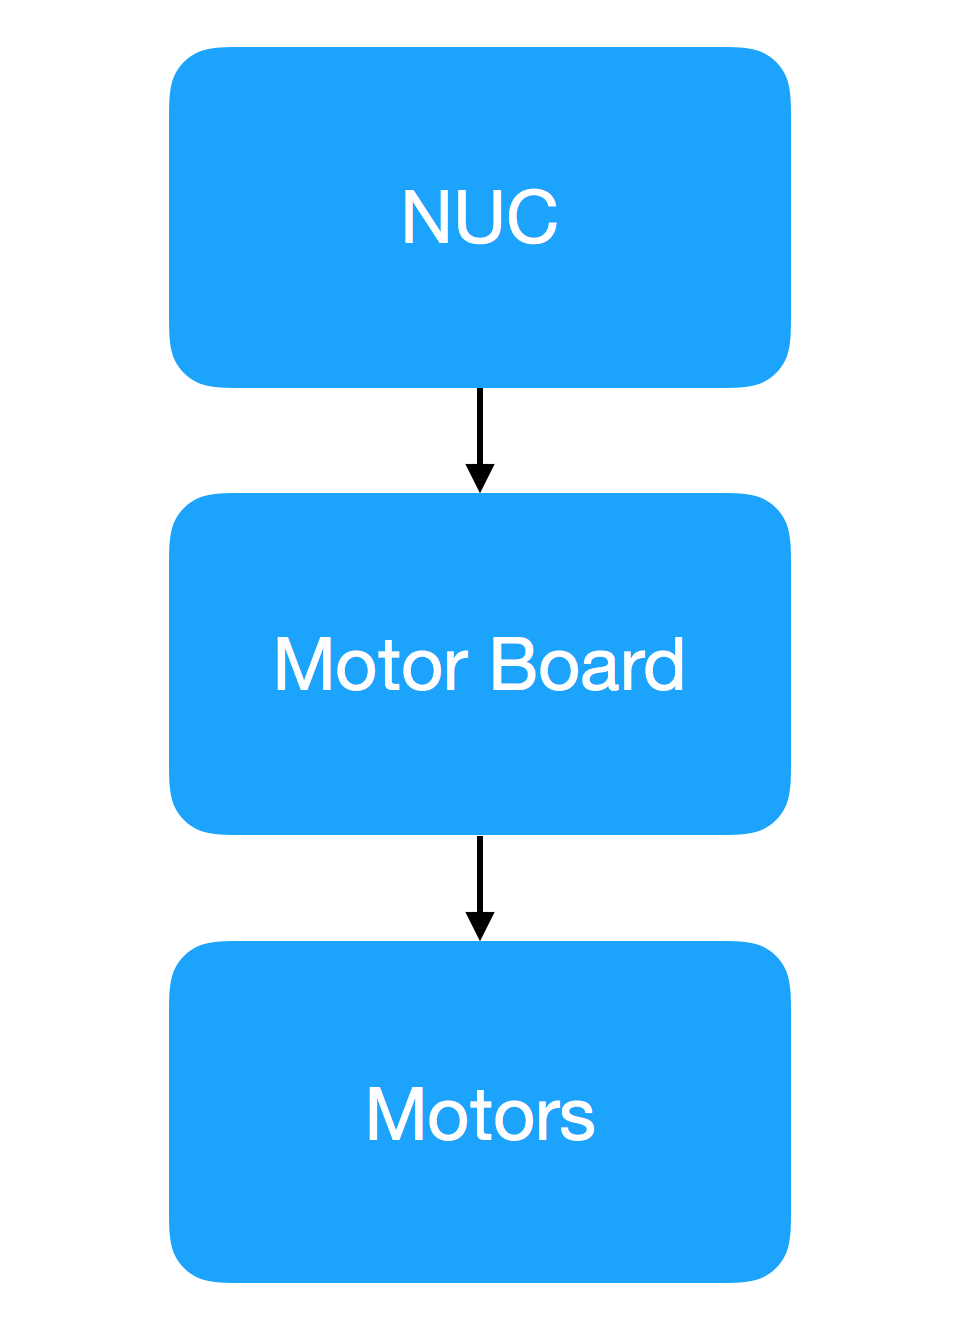
\includegraphics[width=0.7\textwidth]{UpandLow.png}
\caption{motor board's Data Input and Output}
\end{figure}

The primary function of the motor board is to ensure the DC motors are operating at the speed desired by the NUCs. Secondary functions include controlling the LED under-glow, monitoring battery voltage, E-stop status as well as Safety Light. The board also contained two ports for interfacing with OSMCs, a legacy motor controller module RJ IGVC team used in the past. Each functioning circuits can operate independently from each other. \vspace{6pt}\\

\begin{figure}[h]
\centering

\includegraphics[width=0.5\textwidth]{ARMLogo.png}
\caption{ARM logo}
\end{figure}

The motor board is controlled by an mbed NXP LPC1768 microcontroller (referred as mbed in the following). More details here: \url{https://os.mbed.com/platforms/mbed-LPC1768/} \vspace{6pt}\\
\pagebreak

\section{Hardware}
The motor board is designed using AutoDesk EagleCAD. All PCB design files can be found under \url{https://github.com/RoboJackets/igvc-electrical/tree/master/motor board}
\subsection{Power System}
Four voltage level runs through this board. 
\begin{table}[h]
\caption{Summary of functions of Voltage Levels}
\centering
\begin{tabular}{p{3cm}p{4cm}p{4cm}}
\toprule
Level ($V$)  & Direct Input Source & Maximum Ampere \\
\midrule
24V  & Lithium Battery & ? \\
12V  & 12V Rail & 3A  \\
5V  & 12-5 Regulator & 1A \\
3V3 & 5-3.3 Regulator & 300mA \\
\bottomrule
\end{tabular}
\end{table}

24V does not have a power plane on the motor board. The sole purpose of having 24V running through this board is for battery voltage monitor. 24V will be divided between a 4.7k and a 510 ohm resistor to achieve a voltage level of maximum 2.34V. The mbed reads in this value from Analog pin p20 to monitor the battery voltage. $V_{batt} = V_{in} * 3.3 \times (4700 + 510) / 510$. \\

12V plane is the main power source for the motor board. 12V plane powers the 5V plane via 12V-5V regulator (T1). Port to LED underglow, flood light and safety light resides on this power plane. Each with components of enough ampere rating. \\

5V plane powers the mbed, encoder and the USB port to the NUC. 5V plane powers the 3V3 plane via the 5V-3V3 regulator, while the 3V3 plane only powers the imu and the ethernet port. \\

\begin{figure}[h]
\centering
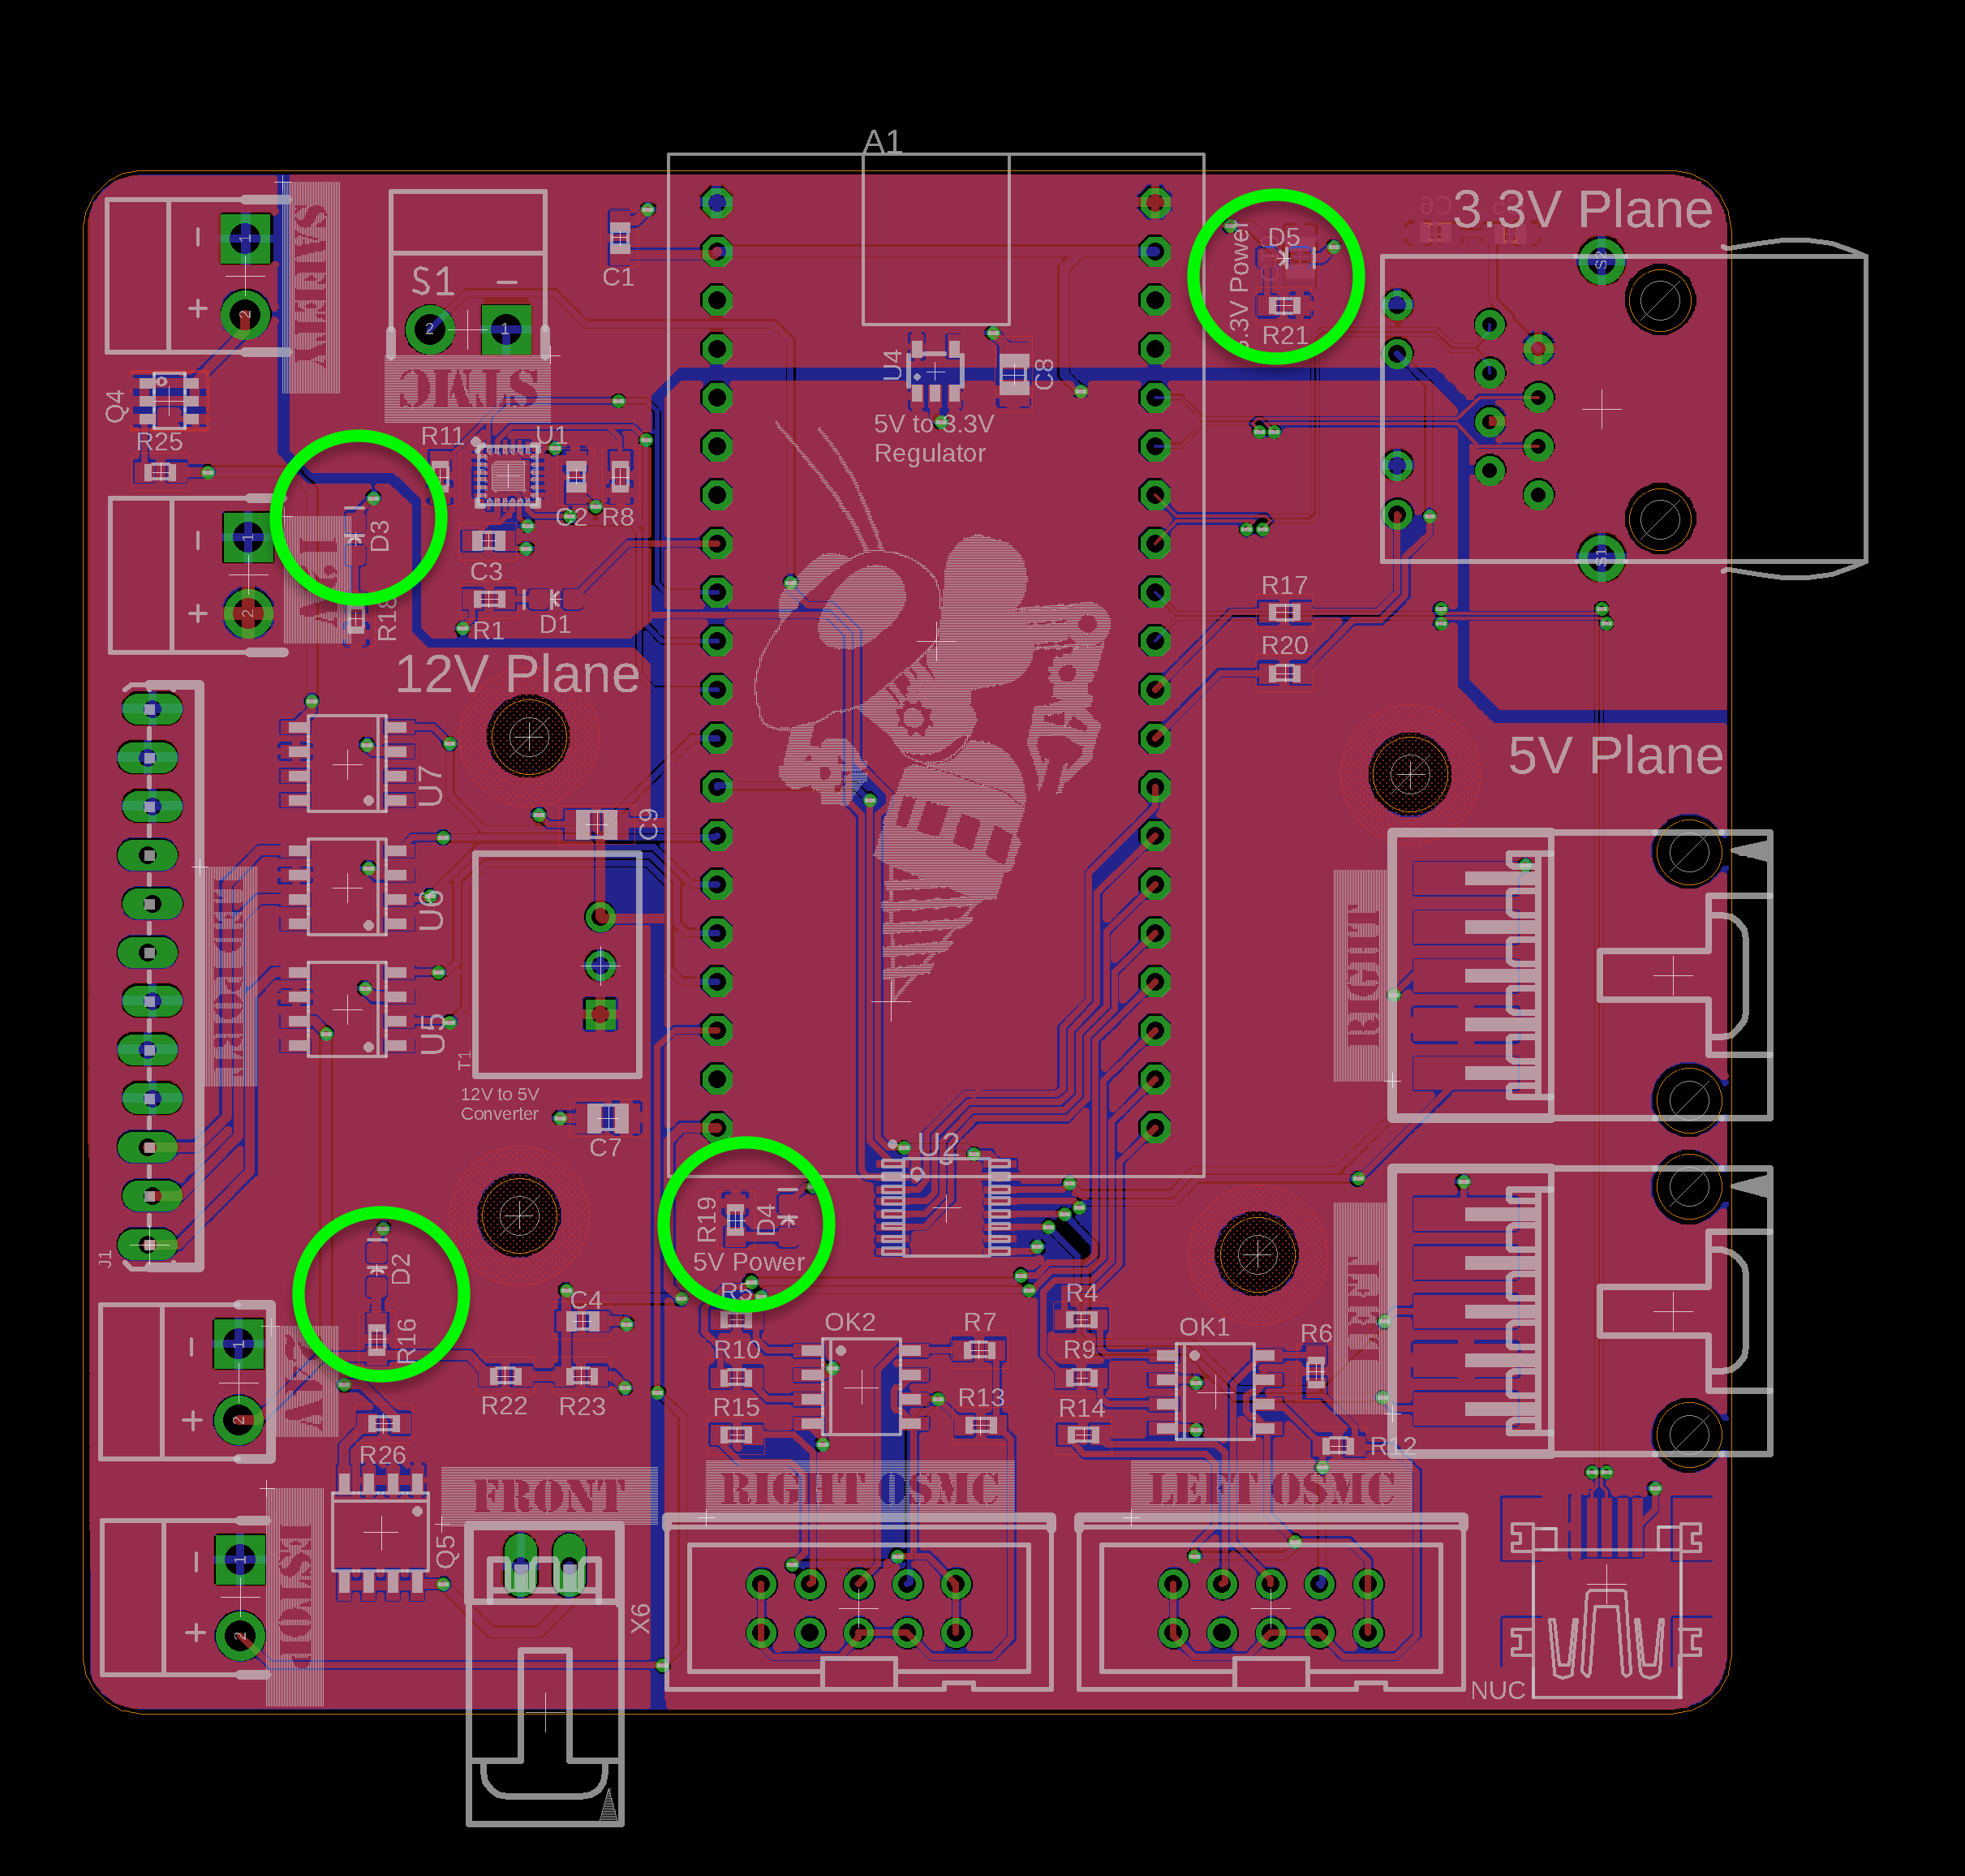
\includegraphics[width=0.8\textwidth]{LED_Indicator.png}
\caption{Power Indictor Circled Out}
\end{figure}

Each power plane has a dedicated LED indicator, indicating that this specific power plane has been powered up. Notice that when USB(either to mbed or X1 port) is connected, without 12V power, 12V LED may still light up. This is caused by the internal design of 12-5 regulator. The fact that 12V LED will light up only dimly suggest that 12V plane does not run 12V at this point. It is discouraged to power the motor board solely by the mbed or USB port.

\subsection{Motor Control}
Motor board interface with a separate motor controller to control the IGVC motors. Motor board itself does not run any high power current through the board. Motors on the IGVC robot is controlled by the Sabertooth 2x60 A motor controller. Data sheets can be found here: \url{https://www.dimensionengineering.com/products/sabertooth2x60}.\\

Motor board communicate with Sabertooth motor controller via a one-line serial communication (the "Simplified Serial Communication" Mode). Only \emph{tx} line on mbed is used, Sabertooth does not send back any data and \emph{rx} line on mbed may leave as not connected and used for other purposes.\\

Port S1 is used for connection to sabertooth motor controller. The serial line connects to port S1 on the sabertooth motor controller. For switch and other specific configurations, please refer to the Sabertooth data sheet listed earlier. \\

\subsection{Light Control}
Motor board controls the indicator light and under-glow light bar.\\

The indicator light is required by the competition rule that it should display different pattern with regards to whether the robot is powered on or not and in autonomous mode or not. Motor board is capable of controlling such a light via port marked "SAFETY". The control signal, however, will come directly from NUC, since it can be implemented easier on NUC.\\

The under-glow light bar can be controlled directly via motor board. The under-glow is purely an aesthetic feature of the robot. Motor board have control over RGB values via PWMOut pins, (see schematics). The board has been designed to handle the current required.

\pagebreak

\section{Firmware}
\subsection{Interacting with NUC}
Motor board communicates with NUC via Serial communication emulated by USBSerial interface. For more details, please see mbed OS 5 API. Serial communication via the onboard USB port \\

Motor board accepts a number of commands from NUC. For most of the time, ($20Hz$ and nonstop), NUC will be sending motor commands; at the startup of ROS, NUC would send command to set parameters for PID algorithm. The list of commands can be found in the following table, any character in parenthesis is optional. When the source is NUC, it's always setting the value in motor board. When the source is motor board, it's always returning a value to the NUC.\\

Motor board abbreviated as MB
\begin{table}[h]
\caption{Summary of Serial Communication}
\centering
    \begin{tabular}{ c  c  c  c  c}
    \toprule
    Preamble & Format & Example & Source & Function \\
    \midrule
    \textdollar & \textdollar(-)X.X,(-)X.X & \textdollar-1.2,1.3 & NUC & Motor speed \\ 
    \#L & \#LX & \#L1 & NUC & Indicator light \\
    \#P & \#PX.X,X.X & \#P8.0,8.0 & NUC & PID P value \\
    \#D & \#DX.X,X.X & \#D8.0,8.0 & NUC & PID D value \\
    \textdollar & 
    \begin{tabular}{@{}c@{}}
        \textdollar(-)X.XX,\\(-)X.XX,0.XXX 
    \end{tabular}
    & 
    \begin{tabular}{@{}c@{}}
        \textdollar-1.25,1.13\\,0.051 
    \end{tabular}
    & MB & Real speed \& $dT$ \\
    \#V & \#VXX.XX,X & \#V24.23,1 & MB & Battery and Estop\\
    \bottomrule
    \end{tabular}
\end{table}

When the communication is directly related to motor, the first value will always be for left motor and second for right. For example \textdollar1.2,-1.3 from NUC means the NUC want to set left motor be at $1.2 m/s$ and right motor at reverse $-1.3 m/s$. \\

\subsection{Controlling the board}
\subsubsection{PID Algorithm}
For software team to have a reliable localization, control over exact speed of motors are required.\\

Such control is done through PID algorithm in the motor board. PID stands for Proportional-Integral-Derivative controller. It operates on the idea that the output is changed based on the proportional, derivative and integral of difference between desired speed and actual speed over a certain $dT$. Details see \url{https://en.wikipedia.org/wiki/PID_controller}\\

Parameter values P, I and D need to be tuned for every different system. Increase proportional term value will increase the speed of the control system response, but will enlarge the overshoot and cause oscillation. Increase derivative term will cause the control system to react more strongly to changes in the error term, but will make the system unstable if the feedback signal is noisy. Increase integral term will sum overtime and drive the Steady-state error to zero, but will also increase the risk of a phenomenon called integral windup. \\

In short, PID need to be tuned, manually, especially if you're reading this document, since the robot probably has gone through a major remake and the system transfer function for the gear box + robot has changed.

\subsubsection{Emergency Stop}
In the event of IGVC robot goes terminator, absolute control over motor is required.\\

Emergency stop is the hardware stop for our robot that will physically cut power to motors, done via a solenoid with diode magic circuits. The significance of Estop to the motor board is that if the motors are cut power and motor board is still running PID algorithm, PID will think power increase is not resulting in reduction of error, thus increase power output and eventually reach maximum. When the robot is re-enabled, such error may cause robot to tip over. \\

A port is added to the motor board to accommodate this issue. Port marked "Estop" is for monitoring estop status. In current electrical system design, when robot is stoped, this port will receive a +5V signal and will be left floating when robot is enabled. This floating signal is complemented by mbed pin's internal pull down configuration. 

\section{Miscellaneous}
\subsection{Legacy Interfaces}
IGVC robot Woodi (Year 2016 - 2017) and her predecessors used 4 Open Source Motor Controller (Referred as OSMC in the following) to control its motors. Current IGVC robot Jessi no longer uses OSMCs, yet a legacy port is reserved on the motor board in case for any unexpected incident. \vspace{6pt}\\
OSMCs are essentially H-bridge DC motor control circuits. Due to the specific design of OSMC, both switches on the high side of H-bridge are hard-wired to \textbf{CLOSED}. Therefore speed and direction control solely depends on the value of low side switches (see OSMC datasheet for specific control logic). The mbed has direct control over the low-side switches via PWMOut pins from p21 to p24. Be advised that one should \textbf{NEVER} set two low switches on the same H bridge to \textbf{CLOSED} at \textbf{ANY TIME}. \vspace{6pt}\\
The motor board used 2 Optoisolators chips to help control the low-side switches. Optoisolators keeps the motor board circuits electrically separated from the motor power circuits. Such design helps to protect the mbed from the fluctuation caused by motors. Although \emph{technically}, the mbed and the motor will still share the same ground, having them not directly electrically connected through the motor board gives more time for the rest of the system to damp the fluctuation and protect the mbed. \vspace{6pt}\\
OSMC datasheets can be found here: \url{http://www.robotpower.com/downloads/osmc3-22sch-clean.pdf}\\

\subsection{Expected Future Usage}
The motor board contains hardware feature not currently utilized. The Ethernet port (X7) is not currently used and the USB port (X1) is only used as Serial port, implemented as USBSerial in mbed firmware. The routing for traces connecting both port to the mbed have followed the layout rules for differential pair. If higher speed communication between the motor board and on-board computer is desired, these ports may be used.

\section{Special Regards}
The author would like to thank Evan Peterson and Ryo Osawa from RoboJackets RoboCup team offered great help in reviewing the design of board and offered much helpful advice. He would also like to thank Jason Gibson from RoboJackets IGVC software team for his time in debugging Serial communication problems with NUC.  
\end{document}